\documentclass[]{article}
\usepackage{lmodern}
\usepackage{amssymb,amsmath}
\usepackage{ifxetex,ifluatex}
\usepackage{fixltx2e} % provides \textsubscript
\ifnum 0\ifxetex 1\fi\ifluatex 1\fi=0 % if pdftex
  \usepackage[T1]{fontenc}
  \usepackage[utf8]{inputenc}
\else % if luatex or xelatex
  \ifxetex
    \usepackage{mathspec}
  \else
    \usepackage{fontspec}
  \fi
  \defaultfontfeatures{Ligatures=TeX,Scale=MatchLowercase}
\fi
% use upquote if available, for straight quotes in verbatim environments
\IfFileExists{upquote.sty}{\usepackage{upquote}}{}
% use microtype if available
\IfFileExists{microtype.sty}{%
\usepackage{microtype}
\UseMicrotypeSet[protrusion]{basicmath} % disable protrusion for tt fonts
}{}
\usepackage[margin=1in]{geometry}
\usepackage{hyperref}
\hypersetup{unicode=true,
            pdftitle={Laborator 2},
            pdfborder={0 0 0},
            breaklinks=true}
\urlstyle{same}  % don't use monospace font for urls
\usepackage{color}
\usepackage{fancyvrb}
\newcommand{\VerbBar}{|}
\newcommand{\VERB}{\Verb[commandchars=\\\{\}]}
\DefineVerbatimEnvironment{Highlighting}{Verbatim}{commandchars=\\\{\}}
% Add ',fontsize=\small' for more characters per line
\usepackage{framed}
\definecolor{shadecolor}{RGB}{248,248,248}
\newenvironment{Shaded}{\begin{snugshade}}{\end{snugshade}}
\newcommand{\KeywordTok}[1]{\textcolor[rgb]{0.13,0.29,0.53}{\textbf{#1}}}
\newcommand{\DataTypeTok}[1]{\textcolor[rgb]{0.13,0.29,0.53}{#1}}
\newcommand{\DecValTok}[1]{\textcolor[rgb]{0.00,0.00,0.81}{#1}}
\newcommand{\BaseNTok}[1]{\textcolor[rgb]{0.00,0.00,0.81}{#1}}
\newcommand{\FloatTok}[1]{\textcolor[rgb]{0.00,0.00,0.81}{#1}}
\newcommand{\ConstantTok}[1]{\textcolor[rgb]{0.00,0.00,0.00}{#1}}
\newcommand{\CharTok}[1]{\textcolor[rgb]{0.31,0.60,0.02}{#1}}
\newcommand{\SpecialCharTok}[1]{\textcolor[rgb]{0.00,0.00,0.00}{#1}}
\newcommand{\StringTok}[1]{\textcolor[rgb]{0.31,0.60,0.02}{#1}}
\newcommand{\VerbatimStringTok}[1]{\textcolor[rgb]{0.31,0.60,0.02}{#1}}
\newcommand{\SpecialStringTok}[1]{\textcolor[rgb]{0.31,0.60,0.02}{#1}}
\newcommand{\ImportTok}[1]{#1}
\newcommand{\CommentTok}[1]{\textcolor[rgb]{0.56,0.35,0.01}{\textit{#1}}}
\newcommand{\DocumentationTok}[1]{\textcolor[rgb]{0.56,0.35,0.01}{\textbf{\textit{#1}}}}
\newcommand{\AnnotationTok}[1]{\textcolor[rgb]{0.56,0.35,0.01}{\textbf{\textit{#1}}}}
\newcommand{\CommentVarTok}[1]{\textcolor[rgb]{0.56,0.35,0.01}{\textbf{\textit{#1}}}}
\newcommand{\OtherTok}[1]{\textcolor[rgb]{0.56,0.35,0.01}{#1}}
\newcommand{\FunctionTok}[1]{\textcolor[rgb]{0.00,0.00,0.00}{#1}}
\newcommand{\VariableTok}[1]{\textcolor[rgb]{0.00,0.00,0.00}{#1}}
\newcommand{\ControlFlowTok}[1]{\textcolor[rgb]{0.13,0.29,0.53}{\textbf{#1}}}
\newcommand{\OperatorTok}[1]{\textcolor[rgb]{0.81,0.36,0.00}{\textbf{#1}}}
\newcommand{\BuiltInTok}[1]{#1}
\newcommand{\ExtensionTok}[1]{#1}
\newcommand{\PreprocessorTok}[1]{\textcolor[rgb]{0.56,0.35,0.01}{\textit{#1}}}
\newcommand{\AttributeTok}[1]{\textcolor[rgb]{0.77,0.63,0.00}{#1}}
\newcommand{\RegionMarkerTok}[1]{#1}
\newcommand{\InformationTok}[1]{\textcolor[rgb]{0.56,0.35,0.01}{\textbf{\textit{#1}}}}
\newcommand{\WarningTok}[1]{\textcolor[rgb]{0.56,0.35,0.01}{\textbf{\textit{#1}}}}
\newcommand{\AlertTok}[1]{\textcolor[rgb]{0.94,0.16,0.16}{#1}}
\newcommand{\ErrorTok}[1]{\textcolor[rgb]{0.64,0.00,0.00}{\textbf{#1}}}
\newcommand{\NormalTok}[1]{#1}
\usepackage{graphicx,grffile}
\makeatletter
\def\maxwidth{\ifdim\Gin@nat@width>\linewidth\linewidth\else\Gin@nat@width\fi}
\def\maxheight{\ifdim\Gin@nat@height>\textheight\textheight\else\Gin@nat@height\fi}
\makeatother
% Scale images if necessary, so that they will not overflow the page
% margins by default, and it is still possible to overwrite the defaults
% using explicit options in \includegraphics[width, height, ...]{}
\setkeys{Gin}{width=\maxwidth,height=\maxheight,keepaspectratio}
\IfFileExists{parskip.sty}{%
\usepackage{parskip}
}{% else
\setlength{\parindent}{0pt}
\setlength{\parskip}{6pt plus 2pt minus 1pt}
}
\setlength{\emergencystretch}{3em}  % prevent overfull lines
\providecommand{\tightlist}{%
  \setlength{\itemsep}{0pt}\setlength{\parskip}{0pt}}
\setcounter{secnumdepth}{5}
% Redefines (sub)paragraphs to behave more like sections
\ifx\paragraph\undefined\else
\let\oldparagraph\paragraph
\renewcommand{\paragraph}[1]{\oldparagraph{#1}\mbox{}}
\fi
\ifx\subparagraph\undefined\else
\let\oldsubparagraph\subparagraph
\renewcommand{\subparagraph}[1]{\oldsubparagraph{#1}\mbox{}}
\fi

%%% Use protect on footnotes to avoid problems with footnotes in titles
\let\rmarkdownfootnote\footnote%
\def\footnote{\protect\rmarkdownfootnote}

%%% Change title format to be more compact
\usepackage{titling}

% Create subtitle command for use in maketitle
\newcommand{\subtitle}[1]{
  \posttitle{
    \begin{center}\large#1\end{center}
    }
}

\setlength{\droptitle}{-2em}
  \title{Laborator 2}
  \pretitle{\vspace{\droptitle}\centering\huge}
  \posttitle{\par}
\subtitle{Intervale de încredere}
  \author{}
  \preauthor{}\postauthor{}
  \date{}
  \predate{}\postdate{}

\usepackage{booktabs}
\usepackage{longtable}
\usepackage{framed,color}
\definecolor{shadecolor}{RGB}{248, 248, 248}
%\definecolor{shadecolor1}{RGB}{216,225,235}
%\definecolor{framecolor}{RGB}{108,123,13}

%\definecolor{shadecolor}{RGB}{226, 255, 241}
\definecolor{shadecolor1}{RGB}{217,225,199}
\definecolor{framecolor}{RGB}{60,179,113}

\ifxetex
  \usepackage{letltxmacro}
  \setlength{\XeTeXLinkMargin}{1pt}
  \LetLtxMacro\SavedIncludeGraphics\includegraphics
  \def\includegraphics#1#{% #1 catches optional stuff (star/opt. arg.)
    \IncludeGraphicsAux{#1}%
  }%
  \newcommand*{\IncludeGraphicsAux}[2]{%
    \XeTeXLinkBox{%
      \SavedIncludeGraphics#1{#2}%
    }%
  }%
\fi

\newenvironment{frshaded*}{%
  \def\FrameCommand{\fboxrule=\FrameRule\fboxsep=\FrameSep \fcolorbox{framecolor}{shadecolor1}}%
  \MakeFramed {\advance\hsize-\width \FrameRestore}}%
{\endMakeFramed}

\newenvironment{rmdblock}[1]
  {\begin{frshaded*}
  \begin{itemize}
  \renewcommand{\labelitemi}{
    \raisebox{-.7\height}[0pt][0pt]{
      {\setkeys{Gin}{width=2em,keepaspectratio}\includegraphics{images/icons/#1}}
    }
  }
  \item
  }
  {
  \end{itemize}
  \end{frshaded*}
  }

\newenvironment{rmdcaution}
  {\begin{rmdblock}{caution}}
  {\end{rmdblock}}
% \newenvironment{rmdinsight}
%   {\begin{rmdblock}{insight}}
%   {\end{rmdblock}}
\newenvironment{rmdexercise}
  {\begin{rmdblock}{exercise}}
  {\end{rmdblock}}
\newenvironment{rmdtip}
  {\begin{rmdblock}{tip}}
  {\end{rmdblock}}


%%%%%%%%%%%%%%%%%%%%%%%%%%%%%%%%%%%%%%%%%%%%%%%%%%%%%%%%%%%%%%%%%%%%%%%%%%%%%%%%%%%%%%%%%%%%%%%%%%%%%%%%%%%%%%%%%%%%%
%%%%%%%%%%% For insight block %%%%%%%%%%%%%%%%%%%%%%%%%%
\definecolor{shadecolor_insight}{RGB}{223,240,216}
\definecolor{framecolor_insight}{RGB}{136,193,137}

%\definecolor{shadecolor_insight}{RGB}{217,225,199}
%\definecolor{framecolor_insight}{RGB}{60,179,113}

\newenvironment{frshaded_insight*}{%
  \def\FrameCommand{\fboxrule=\FrameRule\fboxsep=\FrameSep \fcolorbox{framecolor_insight}{shadecolor_insight}}%
  \MakeFramed {\advance\hsize-\width \FrameRestore}}%
{\endMakeFramed}

\newenvironment{rmdblock_insight}[1]
  {\begin{frshaded_insight*}
  \begin{itemize}
  \renewcommand{\labelitemi}{
    \raisebox{-.7\height}[0pt][0pt]{
      {\setkeys{Gin}{width=2em,keepaspectratio}\includegraphics{images/icons/#1}}
    }
  }
  \item
  }
  {
  \end{itemize}
  \end{frshaded_insight*}
  }

\newenvironment{rmdinsight}
  {\begin{rmdblock_insight}{insight}}
  {\end{rmdblock_insight}}

%%%%%%%%%%%%%%%%%%%%%%%%%%%%%%%%%%%%%%%%%%%%%%%%%%%%%%%%%%%%%%%%%%%%%%%%%%%%%%%%%%%%%%%%%%%%%%%%%%%%%%%%%%%%%%%%%%%%%
\usepackage{subfigure}
\usepackage{booktabs}
\usepackage{slashbox}
\usepackage{color}
%%%%%%%%%%%%%%%%%%%%%%%%%%%%%%%%%%%%%%%%%%%%%%%%%%%%%%%%%%%%%%%%%%%%%%%%%%%%%%%%%%%%%%%%%%%%%%%%%%%%%%%%%%%%%%%%%%%%%
%CITEVA DEFINITII
\def\om{\omega}
\def\Om{\Omega}
\def\et{\eta}
\def\td{\tilde{\delta}}
\def\m{{\mu}}
\def\n{{\nu}}
\def\k{{\kappa}}
\def\l{{\lambda}}
\def\L{{\Lambda}}
\def\g{{\gamma}}
\def\a{{\alpha}}
\def\e{{\varepsilon}}
\def\b{{\beta}}
\def\G{{\Gamma}}
\def\d{{\delta}}
\def\D{{\Delta}}
\def\t{{\theta}}
\def\s{{\sigma}}
\def\S{{\Sigma}}
\def\z{{\zeta}}
\def\qed{\hfill\Box}
\def\ds{\displaystyle}
\def\mc{\mathcal}
%%%%%%%%%%%%%%%%%%%%%%%%%%%%%%%%%%%%%%%%%%%%%%%%%%%%%%%%%%%%%%%%%%%%%%%%%%%%%%%%%%%%%%%%%%%%%%%%%%%%%%%%%%%%%%%%%%%%%%
\def\1{{\mathbf 1}}
\def\CC{{\mathbb C}}
\def\VV{{\mathbb V}}
\def\RR{{\mathbb R}}
\def\QQ{{\mathbb Q}}
\def\ZZ{{\mathbb Z}}
\def\PP{{\mathbb P}}
\def\EE{{\mathbb E}}
\def\NN{{\mathbb N}}
\def\FF{{\mathbb F}}
%\def\SS{{\mathbb S}}
\def\MA{{\mathcal A}}
\def\MO{{\mathcal O}}
\def\MF{{\mathcal F}}
\def\ME{{\mathcal E}}
\def\MR{{\mathcal R}}
\def\MB{{\mathcal B}}
\def\MM{{\mathcal M}}
\def\MN{{\mathcal N}}
\def\MU{{\mathcal U}}
\def\MP{{\mathcal P}}
\def\MS{{\mathcal S}}
\def\MBS{{\mathbf S}}
\def\MX{{\bm{ \mathscr X}}}

% independent sign
\newcommand\independent{\protect\mathpalette{\protect\independenT}{\perp}}
\def\independenT#1#2{\mathrel{\rlap{$#1#2$}\mkern2mu{#1#2}}}

\renewcommand\tablename{Tab.}
\renewcommand{\figurename}{Fig.}

%%%%%%%%%%%%%%%%%%%%%%%%%%%%%%%%%%%%%%%%%%%%%%%%%%%%%%%%%%%%%%%%%%%%%%%%%%%%%%%%%%%%%%%%%%%%%%%%%%%%%%%%%%%%%%%%%%%%%
%Header and Footer
\usepackage{fancyhdr}

\pagestyle{fancy}
\fancyhf{}
\rhead{Universitatea din Bucure\c sti\\ Facultatea de Matematic\u a \c si Informatic\u a}
\lhead{\textit{Curs}: Instrumente Statistice pentru Finan\c te\\ \textit{Instructor}: A. Am\u arioarei}
\rfoot{Pagina \thepage}
\lfoot{Grupa: 403}
%%%%%%%%%%%%%%%%%%%%%%%%%%%%%%%%%%%%%%%
\usepackage{booktabs}
\usepackage{longtable}
\usepackage{array}
\usepackage{multirow}
\usepackage[table]{xcolor}
\usepackage{wrapfig}
\usepackage{float}
\usepackage{colortbl}
\usepackage{pdflscape}
\usepackage{tabu}
\usepackage{threeparttable}
\usepackage[normalem]{ulem}

\begin{document}
\maketitle

%%%%%%%%%%%%%%%%%%%%%%%%
\thispagestyle{fancy}

Obiectivul acestui laborator este de a ilustra noțiunea de interval de
încredere și a face o serie de exemple.

\section{Ilustrarea intervalelor de încredere pentru o populație
normală}\label{ilustrarea-intervalelor-de-incredere-pentru-o-populatie-normala}

Generarea intervalelor de încredere:

\begin{Shaded}
\begin{Highlighting}[]
\CommentTok{# cate panouri sa avem }
\NormalTok{p =}\StringTok{ }\DecValTok{5}

\CommentTok{# nr de intervale de incredere per panou}
\NormalTok{n =}\StringTok{ }\DecValTok{20}

\CommentTok{# talia esantionului}
\NormalTok{m =}\StringTok{ }\DecValTok{50} 

\CommentTok{# coeficient de incredere}
\NormalTok{alpha =}\StringTok{ }\FloatTok{0.05} 

\CommentTok{# media si sd populatia normala}
\NormalTok{mu =}\StringTok{ }\FloatTok{3.5}
\NormalTok{sd =}\StringTok{ }\FloatTok{1.5}

\NormalTok{lo3 <-}\StringTok{ }\NormalTok{hi3 <-}\StringTok{ }\NormalTok{lo2 <-}\StringTok{ }\NormalTok{hi2 <-}\StringTok{ }\NormalTok{lo <-}\StringTok{ }\NormalTok{hi <-}\StringTok{ }\KeywordTok{vector}\NormalTok{(}\StringTok{"list"}\NormalTok{, p)}

\ControlFlowTok{for}\NormalTok{(i }\ControlFlowTok{in} \DecValTok{1}\OperatorTok{:}\NormalTok{p) \{}
\NormalTok{  dat =}\StringTok{ }\KeywordTok{matrix}\NormalTok{(}\KeywordTok{rnorm}\NormalTok{(n}\OperatorTok{*}\NormalTok{m, }\DataTypeTok{mean =}\NormalTok{ mu, }\DataTypeTok{sd =}\NormalTok{ sd), }\DataTypeTok{ncol =}\NormalTok{ m)}
  
  \CommentTok{# media si vaianta esantionului }
\NormalTok{  me =}\StringTok{ }\KeywordTok{apply}\NormalTok{(dat,}\DecValTok{1}\NormalTok{,mean)}
\NormalTok{  se =}\StringTok{ }\KeywordTok{apply}\NormalTok{(dat,}\DecValTok{1}\NormalTok{,sd)}
  
  \CommentTok{# calcul intervale de incredere}
\NormalTok{  lo[[i]] =}\StringTok{ }\NormalTok{me }\OperatorTok{-}\StringTok{ }\KeywordTok{qnorm}\NormalTok{(}\DecValTok{1}\OperatorTok{-}\NormalTok{alpha}\OperatorTok{/}\DecValTok{2}\NormalTok{)}\OperatorTok{*}\NormalTok{sd}\OperatorTok{/}\KeywordTok{sqrt}\NormalTok{(m)}
\NormalTok{  hi[[i]] =}\StringTok{ }\NormalTok{me }\OperatorTok{+}\StringTok{ }\KeywordTok{qnorm}\NormalTok{(}\DecValTok{1}\OperatorTok{-}\NormalTok{alpha}\OperatorTok{/}\DecValTok{2}\NormalTok{)}\OperatorTok{*}\NormalTok{sd}\OperatorTok{/}\KeywordTok{sqrt}\NormalTok{(m)}
  
\NormalTok{  lo2[[i]] =}\StringTok{ }\NormalTok{me }\OperatorTok{-}\StringTok{ }\KeywordTok{qnorm}\NormalTok{(}\DecValTok{1}\OperatorTok{-}\NormalTok{alpha}\OperatorTok{/}\DecValTok{2}\NormalTok{)}\OperatorTok{*}\NormalTok{se}\OperatorTok{/}\KeywordTok{sqrt}\NormalTok{(m)}
\NormalTok{  hi2[[i]] =}\StringTok{ }\NormalTok{me }\OperatorTok{+}\StringTok{ }\KeywordTok{qnorm}\NormalTok{(}\DecValTok{1}\OperatorTok{-}\NormalTok{alpha}\OperatorTok{/}\DecValTok{2}\NormalTok{)}\OperatorTok{*}\NormalTok{se}\OperatorTok{/}\KeywordTok{sqrt}\NormalTok{(m)}
  
\NormalTok{  lo3[[i]] =}\StringTok{ }\NormalTok{me }\OperatorTok{-}\StringTok{ }\KeywordTok{qt}\NormalTok{(}\DecValTok{1}\OperatorTok{-}\NormalTok{alpha}\OperatorTok{/}\DecValTok{2}\NormalTok{, m}\OperatorTok{-}\DecValTok{1}\NormalTok{)}\OperatorTok{*}\NormalTok{se}\OperatorTok{/}\KeywordTok{sqrt}\NormalTok{(m)}
\NormalTok{  hi3[[i]] =}\StringTok{ }\NormalTok{me }\OperatorTok{+}\StringTok{ }\KeywordTok{qt}\NormalTok{(}\DecValTok{1}\OperatorTok{-}\NormalTok{alpha}\OperatorTok{/}\DecValTok{2}\NormalTok{, m}\OperatorTok{-}\DecValTok{1}\NormalTok{)}\OperatorTok{*}\NormalTok{se}\OperatorTok{/}\KeywordTok{sqrt}\NormalTok{(m)}
\NormalTok{\}}
\end{Highlighting}
\end{Shaded}

Intervale de încredere atunci când \(\sigma\) este cunoscut:

\begin{Shaded}
\begin{Highlighting}[]
\NormalTok{r =}\StringTok{ }\KeywordTok{range}\NormalTok{(}\KeywordTok{unlist}\NormalTok{(}\KeywordTok{c}\NormalTok{(lo,hi,lo2,hi2,lo3,hi3)))}

\KeywordTok{par}\NormalTok{(}\DataTypeTok{mfrow=}\KeywordTok{c}\NormalTok{(}\DecValTok{1}\NormalTok{,}\DecValTok{5}\NormalTok{), }\DataTypeTok{las=}\DecValTok{1}\NormalTok{, }\DataTypeTok{mar=}\KeywordTok{c}\NormalTok{(}\FloatTok{5.1}\NormalTok{,}\FloatTok{2.1}\NormalTok{,}\FloatTok{6.1}\NormalTok{,}\FloatTok{2.1}\NormalTok{))}

\ControlFlowTok{for}\NormalTok{(i }\ControlFlowTok{in} \DecValTok{1}\OperatorTok{:}\NormalTok{p) \{}
  \KeywordTok{plot}\NormalTok{(}\DecValTok{0}\NormalTok{, }\DecValTok{0}\NormalTok{, }\DataTypeTok{type=}\StringTok{"n"}\NormalTok{, }
       \DataTypeTok{ylim =} \FloatTok{0.5}\OperatorTok{+}\KeywordTok{c}\NormalTok{(}\DecValTok{0}\NormalTok{,n), }
       \DataTypeTok{xlim =}\NormalTok{ r, }
       \DataTypeTok{ylab =} \StringTok{""}\NormalTok{, }
       \DataTypeTok{xlab =} \StringTok{""}\NormalTok{, }
       \DataTypeTok{yaxt =} \StringTok{"n"}\NormalTok{)}
  
  \KeywordTok{abline}\NormalTok{(}\DataTypeTok{v =}\NormalTok{ mu, }\DataTypeTok{lty=}\DecValTok{2}\NormalTok{, }\DataTypeTok{col=}\StringTok{"brown3"}\NormalTok{, }\DataTypeTok{lwd=}\DecValTok{2}\NormalTok{)}
  
  \KeywordTok{segments}\NormalTok{(lo[[i]], }\DecValTok{1}\OperatorTok{:}\NormalTok{n,}
\NormalTok{           hi[[i]], }\DecValTok{1}\OperatorTok{:}\NormalTok{n,}
           \DataTypeTok{lwd=}\DecValTok{2}\NormalTok{)}
  
\NormalTok{  o =}\StringTok{ }\NormalTok{(}\DecValTok{1}\OperatorTok{:}\NormalTok{n)[lo[[i]] }\OperatorTok{>}\StringTok{ }\FloatTok{3.5} \OperatorTok{|}\StringTok{ }\NormalTok{hi[[i]] }\OperatorTok{<}\StringTok{ }\FloatTok{3.5}\NormalTok{]}
  
  \KeywordTok{segments}\NormalTok{(lo[[i]][o], o,}
\NormalTok{           hi[[i]][o], o,}
           \DataTypeTok{lwd=}\DecValTok{2}\NormalTok{,}\DataTypeTok{col=}\StringTok{"orange"}\NormalTok{)}
\NormalTok{\}}

\KeywordTok{par}\NormalTok{(}\DataTypeTok{mfrow=}\KeywordTok{c}\NormalTok{(}\DecValTok{1}\NormalTok{,}\DecValTok{1}\NormalTok{))}

\KeywordTok{mtext}\NormalTok{(}\KeywordTok{expression}\NormalTok{(}\KeywordTok{paste}\NormalTok{(}\StringTok{"100 intervale de încredere pentru "}\NormalTok{, mu)), }
      \DataTypeTok{side=}\DecValTok{3}\NormalTok{, }\DataTypeTok{cex=}\FloatTok{1.5}\NormalTok{, }\DataTypeTok{xpd=}\OtherTok{TRUE}\NormalTok{, }\DataTypeTok{line=}\DecValTok{4}\NormalTok{)}
\KeywordTok{mtext}\NormalTok{(}\KeywordTok{expression}\NormalTok{(}\KeywordTok{paste}\NormalTok{(}\StringTok{"("}\NormalTok{,sigma,}\StringTok{" cunoscut)"}\NormalTok{)), }\DataTypeTok{side=}\DecValTok{3}\NormalTok{, }\DataTypeTok{cex=}\FloatTok{1.3}\NormalTok{, }
      \DataTypeTok{xpd=}\OtherTok{TRUE}\NormalTok{,}\DataTypeTok{line=}\FloatTok{2.7}\NormalTok{)}
\end{Highlighting}
\end{Shaded}

\begin{center}\includegraphics[width=0.8\linewidth]{Lab_2_files/figure-latex/unnamed-chunk-3-1} \end{center}

Intervale de încredere \textbf{incorecte} atunci când \(\sigma\) nu este
cunoscut:

\begin{Shaded}
\begin{Highlighting}[]
\KeywordTok{par}\NormalTok{(}\DataTypeTok{mfrow=}\KeywordTok{c}\NormalTok{(}\DecValTok{1}\NormalTok{,}\DecValTok{5}\NormalTok{), }\DataTypeTok{las=}\DecValTok{1}\NormalTok{, }\DataTypeTok{mar=}\KeywordTok{c}\NormalTok{(}\FloatTok{5.1}\NormalTok{,}\FloatTok{2.1}\NormalTok{,}\FloatTok{6.1}\NormalTok{,}\FloatTok{2.1}\NormalTok{))}

\ControlFlowTok{for}\NormalTok{(i }\ControlFlowTok{in} \DecValTok{1}\OperatorTok{:}\NormalTok{p) \{}
  \KeywordTok{plot}\NormalTok{(}\DecValTok{0}\NormalTok{, }\DecValTok{0}\NormalTok{,}
       \DataTypeTok{type=}\StringTok{"n"}\NormalTok{,}
       \DataTypeTok{ylim=}\FloatTok{0.5}\OperatorTok{+}\KeywordTok{c}\NormalTok{(}\DecValTok{0}\NormalTok{,n),}
       \DataTypeTok{xlim=}\NormalTok{r,}
       \DataTypeTok{ylab=}\StringTok{""}\NormalTok{,}
       \DataTypeTok{xlab=}\StringTok{""}\NormalTok{,}
       \DataTypeTok{yaxt=}\StringTok{"n"}\NormalTok{)}
  
  \KeywordTok{abline}\NormalTok{(}\DataTypeTok{v =}\NormalTok{ mu,}\DataTypeTok{lty =} \DecValTok{2}\NormalTok{, }\DataTypeTok{col=}\StringTok{"brown3"}\NormalTok{, }\DataTypeTok{lwd=}\DecValTok{2}\NormalTok{)}
  
  \KeywordTok{segments}\NormalTok{(lo2[[i]], }\DecValTok{1}\OperatorTok{:}\NormalTok{n,}
\NormalTok{           hi2[[i]], }\DecValTok{1}\OperatorTok{:}\NormalTok{n,}
           \DataTypeTok{lwd=}\DecValTok{2}\NormalTok{)}
  
\NormalTok{  o =}\StringTok{ }\NormalTok{(}\DecValTok{1}\OperatorTok{:}\NormalTok{n)[lo2[[i]] }\OperatorTok{>}\StringTok{ }\FloatTok{3.5} \OperatorTok{|}\StringTok{ }\NormalTok{hi2[[i]] }\OperatorTok{<}\StringTok{ }\FloatTok{3.5}\NormalTok{]}
  
  \KeywordTok{segments}\NormalTok{(lo2[[i]][o],o,}
\NormalTok{           hi2[[i]][o],o,}
           \DataTypeTok{lwd=}\DecValTok{2}\NormalTok{, }\DataTypeTok{col=}\StringTok{"orange"}\NormalTok{)}
\NormalTok{\}}

\KeywordTok{par}\NormalTok{(}\DataTypeTok{mfrow=}\KeywordTok{c}\NormalTok{(}\DecValTok{1}\NormalTok{,}\DecValTok{1}\NormalTok{))}
\KeywordTok{mtext}\NormalTok{(}\KeywordTok{expression}\NormalTok{(}\KeywordTok{paste}\NormalTok{(}\StringTok{"100 intervale de încredere incorecte pentru "}\NormalTok{, mu)), }
      \DataTypeTok{side=}\DecValTok{3}\NormalTok{, }\DataTypeTok{cex=}\FloatTok{1.5}\NormalTok{, }\DataTypeTok{xpd=}\OtherTok{TRUE}\NormalTok{, }\DataTypeTok{line=}\DecValTok{4}\NormalTok{)}
\KeywordTok{mtext}\NormalTok{(}\KeywordTok{expression}\NormalTok{(}\KeywordTok{paste}\NormalTok{(}\StringTok{"("}\NormalTok{,sigma,}\StringTok{" necunoscut)"}\NormalTok{)),}
      \DataTypeTok{side=}\DecValTok{3}\NormalTok{,}\DataTypeTok{cex=}\FloatTok{1.3}\NormalTok{,}\DataTypeTok{xpd=}\OtherTok{TRUE}\NormalTok{,}\DataTypeTok{line=}\FloatTok{2.7}\NormalTok{)}
\end{Highlighting}
\end{Shaded}

\begin{center}\includegraphics[width=0.8\linewidth]{Lab_2_files/figure-latex/unnamed-chunk-4-1} \end{center}

Intervale de încredere \textbf{corecte} atunci când \(\sigma\) nu este
cunoscut:

\begin{Shaded}
\begin{Highlighting}[]
\KeywordTok{par}\NormalTok{(}\DataTypeTok{mfrow=}\KeywordTok{c}\NormalTok{(}\DecValTok{1}\NormalTok{,}\DecValTok{5}\NormalTok{), }\DataTypeTok{las=}\DecValTok{1}\NormalTok{, }\DataTypeTok{mar=}\KeywordTok{c}\NormalTok{(}\FloatTok{5.1}\NormalTok{,}\FloatTok{2.1}\NormalTok{,}\FloatTok{6.1}\NormalTok{,}\FloatTok{2.1}\NormalTok{))}

\ControlFlowTok{for}\NormalTok{(i }\ControlFlowTok{in} \DecValTok{1}\OperatorTok{:}\NormalTok{p) \{}
  \KeywordTok{plot}\NormalTok{(}\DecValTok{0}\NormalTok{,}\DecValTok{0}\NormalTok{,}
       \DataTypeTok{type=}\StringTok{"n"}\NormalTok{,}
       \DataTypeTok{ylim=}\FloatTok{0.5}\OperatorTok{+}\KeywordTok{c}\NormalTok{(}\DecValTok{0}\NormalTok{,n),}
       \DataTypeTok{xlim=}\NormalTok{r,}
       \DataTypeTok{ylab=}\StringTok{""}\NormalTok{,}
       \DataTypeTok{xlab=}\StringTok{""}\NormalTok{,}
       \DataTypeTok{yaxt=}\StringTok{"n"}\NormalTok{)}
  
  \KeywordTok{abline}\NormalTok{(}\DataTypeTok{v =}\NormalTok{ mu, }\DataTypeTok{lty=}\DecValTok{2}\NormalTok{, }\DataTypeTok{col=}\StringTok{"brown3"}\NormalTok{, }\DataTypeTok{lwd=}\DecValTok{2}\NormalTok{)}
  
  \KeywordTok{segments}\NormalTok{(lo3[[i]],}\DecValTok{1}\OperatorTok{:}\NormalTok{n,}
\NormalTok{           hi3[[i]],}\DecValTok{1}\OperatorTok{:}\NormalTok{n,}
           \DataTypeTok{lwd=}\DecValTok{2}\NormalTok{)}
  
\NormalTok{  o =}\StringTok{ }\NormalTok{(}\DecValTok{1}\OperatorTok{:}\NormalTok{n)[lo3[[i]] }\OperatorTok{>}\StringTok{ }\FloatTok{3.5} \OperatorTok{|}\StringTok{ }\NormalTok{hi3[[i]] }\OperatorTok{<}\StringTok{ }\FloatTok{3.5}\NormalTok{]}
  
  \KeywordTok{segments}\NormalTok{(lo3[[i]][o],o,}
\NormalTok{           hi3[[i]][o],o,}
           \DataTypeTok{lwd=}\DecValTok{2}\NormalTok{, }\DataTypeTok{col=}\StringTok{"orange"}\NormalTok{)}
\NormalTok{\}}
\KeywordTok{par}\NormalTok{(}\DataTypeTok{mfrow=}\KeywordTok{c}\NormalTok{(}\DecValTok{1}\NormalTok{,}\DecValTok{1}\NormalTok{))}

\KeywordTok{mtext}\NormalTok{(}\KeywordTok{expression}\NormalTok{(}\KeywordTok{paste}\NormalTok{(}\StringTok{"100 intervale de încredere pentru "}\NormalTok{, mu)),}
      \DataTypeTok{side=}\DecValTok{3}\NormalTok{, }\DataTypeTok{cex=}\FloatTok{1.5}\NormalTok{, }\DataTypeTok{xpd=}\OtherTok{TRUE}\NormalTok{, }\DataTypeTok{line=}\DecValTok{4}\NormalTok{)}

\KeywordTok{mtext}\NormalTok{(}\KeywordTok{expression}\NormalTok{(}\KeywordTok{paste}\NormalTok{(}\StringTok{"("}\NormalTok{,sigma,}\StringTok{" necunoscut)"}\NormalTok{)),}
      \DataTypeTok{side=}\DecValTok{3}\NormalTok{, }\DataTypeTok{cex=}\FloatTok{1.3}\NormalTok{, }\DataTypeTok{xpd=}\OtherTok{TRUE}\NormalTok{, }\DataTypeTok{line=}\FloatTok{2.7}\NormalTok{)}
\end{Highlighting}
\end{Shaded}

\begin{center}\includegraphics[width=0.8\linewidth]{Lab_2_files/figure-latex/unnamed-chunk-5-1} \end{center}

\section{Ilustrarea probabilității de
acoperire}\label{ilustrarea-probabilitatii-de-acoperire}

\subsection{Intervale de încredere de tip
Wald}\label{intervale-de-incredere-de-tip-wald}

\begin{rmdexercise}
Fie \(X_1,X_2,\ldots,X_n\) un eșantion de talie \(n\) dintr-o populație
Bernoulli de medie \(\theta\). Determinați un interval de încredere
asimptotic pentru \(\theta\) cu un coeficient de încredere \(1-\alpha\).

Ilustrați grafic \emph{probabilitatea de acoperire}
\(\mathbb{P}_{\theta}\left(IC^{1-\alpha}(\theta)\ni \theta\right)\) ca
funcție de \(\theta\) pentru diferite valori ale lui
\(n\in \{50, 100\}\) și \(\alpha = 0.05\). Ce observați?
\end{rmdexercise}

Știm că \(\hat{\theta}_n = \bar{X}_n\) este estimatorul de
verosimilitate maximă pentru \(\theta\) și folosind proprietatea
asimptotică a estimatorilor de verosimilitate maximă găsim că un
interval de încredere asimptotic pentru \(\theta\) este (folosid o
înlocuire de tip Wald)

\[
  IC^{1-\alpha}(\theta) = \bar{X}_n \pm z_{1-\frac{\alpha}{2}}\sqrt{\frac{\bar{X}_n(1-\bar{X}_n)}{n}}.
\]

Probabilitatea de acoperire este:

\begin{Shaded}
\begin{Highlighting}[]
\NormalTok{binom.wald.cvg =}\StringTok{ }\ControlFlowTok{function}\NormalTok{(theta, n, alpha) \{}
\NormalTok{  z =}\StringTok{ }\KeywordTok{qnorm}\NormalTok{(}\DecValTok{1} \OperatorTok{-}\StringTok{ }\NormalTok{alpha }\OperatorTok{/}\StringTok{ }\DecValTok{2}\NormalTok{)}
  
\NormalTok{  f =}\StringTok{ }\ControlFlowTok{function}\NormalTok{(p) \{}
\NormalTok{    t =}\StringTok{ }\DecValTok{0}\OperatorTok{:}\NormalTok{n}

\NormalTok{    s =}\StringTok{ }\KeywordTok{sqrt}\NormalTok{(t }\OperatorTok{*}\StringTok{ }\NormalTok{(n }\OperatorTok{-}\StringTok{ }\NormalTok{t) }\OperatorTok{/}\StringTok{ }\NormalTok{n)}
\NormalTok{    o =}\StringTok{ }\NormalTok{(t }\OperatorTok{-}\StringTok{ }\NormalTok{z }\OperatorTok{*}\StringTok{ }\NormalTok{s }\OperatorTok{<=}\StringTok{ }\NormalTok{n }\OperatorTok{*}\StringTok{ }\NormalTok{p }\OperatorTok{&}\StringTok{ }\NormalTok{t }\OperatorTok{+}\StringTok{ }\NormalTok{z }\OperatorTok{*}\StringTok{ }\NormalTok{s }\OperatorTok{>=}\StringTok{ }\NormalTok{n }\OperatorTok{*}\StringTok{ }\NormalTok{p)}
  
    \KeywordTok{return}\NormalTok{(}\KeywordTok{sum}\NormalTok{(o }\OperatorTok{*}\StringTok{ }\KeywordTok{dbinom}\NormalTok{(t, }\DataTypeTok{size =}\NormalTok{ n, }\DataTypeTok{prob =}\NormalTok{ p)))}
\NormalTok{  \}}
  
\NormalTok{  out =}\StringTok{ }\KeywordTok{sapply}\NormalTok{(theta, f)}
  \KeywordTok{return}\NormalTok{(out)}
\NormalTok{\}}
\end{Highlighting}
\end{Shaded}

\begin{Shaded}
\begin{Highlighting}[]
\CommentTok{# date intrare}
\KeywordTok{par}\NormalTok{(}\DataTypeTok{mfrow =} \KeywordTok{c}\NormalTok{(}\DecValTok{1}\NormalTok{,}\DecValTok{2}\NormalTok{))}

\NormalTok{n =}\StringTok{ }\DecValTok{50}
\NormalTok{alpha =}\StringTok{ }\FloatTok{0.05}

\NormalTok{theta =}\StringTok{ }\KeywordTok{seq}\NormalTok{(}\FloatTok{0.01}\NormalTok{, }\FloatTok{0.99}\NormalTok{, }\DataTypeTok{len=}\DecValTok{200}\NormalTok{)}

\KeywordTok{plot}\NormalTok{(theta, }\KeywordTok{binom.wald.cvg}\NormalTok{(theta, n, alpha), }
     \DataTypeTok{ylim=}\KeywordTok{c}\NormalTok{(}\FloatTok{0.5}\NormalTok{, }\DecValTok{1}\NormalTok{), }\DataTypeTok{type=}\StringTok{"l"}\NormalTok{, }\DataTypeTok{lwd=}\DecValTok{1}\NormalTok{,}
     \DataTypeTok{bty =} \StringTok{"n"}\NormalTok{,}
     \DataTypeTok{col =} \StringTok{"forestgreen"}\NormalTok{, }
     \DataTypeTok{main =} \KeywordTok{paste0}\NormalTok{(}\StringTok{"n = "}\NormalTok{, n),}
     \DataTypeTok{xlab =} \KeywordTok{expression}\NormalTok{(theta), }
     \DataTypeTok{ylab =} \StringTok{"Probabilitatea de acoperire"}\NormalTok{)}

\KeywordTok{abline}\NormalTok{(}\DataTypeTok{h =} \DecValTok{1}\OperatorTok{-}\NormalTok{alpha, }\DataTypeTok{lty=}\DecValTok{3}\NormalTok{, }\DataTypeTok{lwd=}\DecValTok{2}\NormalTok{,}
       \DataTypeTok{col =} \StringTok{"brown3"}\NormalTok{)}

\CommentTok{# al doilea grafic}
\NormalTok{n =}\StringTok{ }\DecValTok{100}

\KeywordTok{plot}\NormalTok{(theta, }\KeywordTok{binom.wald.cvg}\NormalTok{(theta, n, alpha), }
     \DataTypeTok{ylim=}\KeywordTok{c}\NormalTok{(}\FloatTok{0.5}\NormalTok{, }\DecValTok{1}\NormalTok{), }\DataTypeTok{type=}\StringTok{"l"}\NormalTok{, }\DataTypeTok{lwd=}\DecValTok{1}\NormalTok{,}
     \DataTypeTok{bty =} \StringTok{"n"}\NormalTok{,}
     \DataTypeTok{col =} \StringTok{"forestgreen"}\NormalTok{, }
     \DataTypeTok{main =} \KeywordTok{paste0}\NormalTok{(}\StringTok{"n = "}\NormalTok{, n),}
     \DataTypeTok{xlab =} \KeywordTok{expression}\NormalTok{(theta), }
     \DataTypeTok{ylab =} \StringTok{"Probabilitatea de acoperire"}\NormalTok{)}

\KeywordTok{abline}\NormalTok{(}\DataTypeTok{h =} \DecValTok{1}\OperatorTok{-}\NormalTok{alpha, }\DataTypeTok{lty=}\DecValTok{3}\NormalTok{, }\DataTypeTok{lwd=}\DecValTok{2}\NormalTok{,}
       \DataTypeTok{col =} \StringTok{"brown3"}\NormalTok{)}
\end{Highlighting}
\end{Shaded}

\begin{center}\includegraphics[width=0.8\linewidth]{Lab_2_files/figure-latex/unnamed-chunk-8-1} \end{center}

Observăm că probabilitatea de acoperire tinde să fie mai scăzută decât
pragul \(1-\alpha = 0.95\) ales pentru majoritatea valorilor lui
\(\theta\).

\begin{rmdexercise}
Fie \(X_1,X_2,\ldots,X_n\) un eșantion de talie \(n\) dintr-o populație
Exponențială de parametru \(\theta\). Determinați un interval de
încredere asimptotic pentru \(\theta\) cu un coeficient de încredere
\(1-\alpha\).

Ilustrați grafic \emph{probabilitatea de acoperire}
\(\mathbb{P}_{\theta}\left(IC^{1-\alpha}(\theta)\ni \theta\right)\) ca
funcție de \(n\) pentru diferite valori ale lui \(\theta\in \{1, 3\}\)
și \(\alpha = 0.05\). Ce observați?
\end{rmdexercise}

Știm că \(\hat{\theta}_n = \bar{X}_n\) este estimatorul de
verosimilitate maximă pentru \(\theta\) și folosind proprietatea
asimptotică a estimatorilor de verosimilitate maximă găsim că un
interval de încredere asimptotic pentru \(\theta\) este (folosid o
înlocuire de tip Wald)

\[
  IC^{1-\alpha}(\theta) = \bar{X}_n \pm z_{1-\frac{\alpha}{2}}\frac{\bar{X}_n}{\sqrt{n}}.
\]

\begin{Shaded}
\begin{Highlighting}[]
\NormalTok{expo.wald.cvg =}\StringTok{ }\ControlFlowTok{function}\NormalTok{(N, theta, alpha) \{}
\NormalTok{    z =}\StringTok{ }\KeywordTok{qnorm}\NormalTok{(}\DecValTok{1} \OperatorTok{-}\StringTok{ }\NormalTok{alpha }\OperatorTok{/}\StringTok{ }\DecValTok{2}\NormalTok{)}
    
\NormalTok{  f =}\StringTok{ }\ControlFlowTok{function}\NormalTok{(n) \{}
\NormalTok{    f1 =}\StringTok{ }\DecValTok{1} \OperatorTok{-}\StringTok{ }\KeywordTok{pgamma}\NormalTok{(n }\OperatorTok{*}\StringTok{ }\NormalTok{theta }\OperatorTok{/}\StringTok{ }\NormalTok{(}\DecValTok{1} \OperatorTok{-}\StringTok{ }\NormalTok{z }\OperatorTok{/}\StringTok{ }\KeywordTok{sqrt}\NormalTok{(n)), }
                    \DataTypeTok{shape=}\NormalTok{n, }\DataTypeTok{rate=}\DecValTok{1}\OperatorTok{/}\NormalTok{theta)}
\NormalTok{    f2 =}\StringTok{ }\KeywordTok{pgamma}\NormalTok{(n }\OperatorTok{*}\StringTok{ }\NormalTok{theta }\OperatorTok{/}\StringTok{ }\NormalTok{(}\DecValTok{1} \OperatorTok{+}\StringTok{ }\NormalTok{z }\OperatorTok{/}\StringTok{ }\KeywordTok{sqrt}\NormalTok{(n)), }
                \DataTypeTok{shape=}\NormalTok{n, }\DataTypeTok{rate=}\DecValTok{1}\OperatorTok{/}\NormalTok{theta)}
    \KeywordTok{return}\NormalTok{(}\DecValTok{1} \OperatorTok{-}\StringTok{ }\NormalTok{f1 }\OperatorTok{-}\StringTok{ }\NormalTok{f2)}
\NormalTok{  \}}
  
\NormalTok{  out =}\StringTok{ }\KeywordTok{sapply}\NormalTok{(N, f)}
  \KeywordTok{return}\NormalTok{(out)}
\NormalTok{\}}
\end{Highlighting}
\end{Shaded}

\begin{Shaded}
\begin{Highlighting}[]
\NormalTok{alpha =}\StringTok{ }\FloatTok{0.05}
\NormalTok{n =}\StringTok{ }\KeywordTok{seq}\NormalTok{(}\DecValTok{100}\NormalTok{, }\DecValTok{1500}\NormalTok{, }\DataTypeTok{by=}\DecValTok{50}\NormalTok{)}

\KeywordTok{par}\NormalTok{(}\DataTypeTok{mfrow =} \KeywordTok{c}\NormalTok{(}\DecValTok{1}\NormalTok{,}\DecValTok{2}\NormalTok{))}

\KeywordTok{plot}\NormalTok{(n, }\KeywordTok{expo.wald.cvg}\NormalTok{(n, }\DecValTok{1}\NormalTok{, alpha), }
     \DataTypeTok{ylim=}\KeywordTok{c}\NormalTok{(}\FloatTok{0.945}\NormalTok{, }\FloatTok{0.95}\NormalTok{), }\DataTypeTok{type=}\StringTok{"l"}\NormalTok{, }\DataTypeTok{lwd=}\DecValTok{2}\NormalTok{,}
     \DataTypeTok{bty =} \StringTok{"n"}\NormalTok{, }\DataTypeTok{col =} \StringTok{"forestgreen"}\NormalTok{,}
     \DataTypeTok{main =} \KeywordTok{TeX}\NormalTok{(}\StringTok{"$}\CharTok{\textbackslash{}\textbackslash{}}\StringTok{theta = 1$"}\NormalTok{),}
     \DataTypeTok{xlab=}\StringTok{"n"}\NormalTok{, }\DataTypeTok{ylab=}\StringTok{"Probabilitatea de acoperire"}\NormalTok{)}

\KeywordTok{abline}\NormalTok{(}\DataTypeTok{h=}\DecValTok{1}\OperatorTok{-}\NormalTok{alpha, }\DataTypeTok{lty=}\DecValTok{3}\NormalTok{, }\DataTypeTok{lwd=}\DecValTok{2}\NormalTok{,}
       \DataTypeTok{col =} \StringTok{"brown3"}\NormalTok{)}

\KeywordTok{plot}\NormalTok{(n, }\KeywordTok{expo.wald.cvg}\NormalTok{(n, }\DecValTok{3}\NormalTok{, alpha), }
     \DataTypeTok{ylim=}\KeywordTok{c}\NormalTok{(}\FloatTok{0.945}\NormalTok{, }\FloatTok{0.95}\NormalTok{), }\DataTypeTok{type=}\StringTok{"l"}\NormalTok{, }\DataTypeTok{lwd=}\DecValTok{2}\NormalTok{,}
     \DataTypeTok{bty =} \StringTok{"n"}\NormalTok{, }\DataTypeTok{col =} \StringTok{"forestgreen"}\NormalTok{,}
     \DataTypeTok{main =} \KeywordTok{TeX}\NormalTok{(}\StringTok{"$}\CharTok{\textbackslash{}\textbackslash{}}\StringTok{theta = 3$"}\NormalTok{),}
     \DataTypeTok{xlab=}\StringTok{"n"}\NormalTok{, }\DataTypeTok{ylab=}\StringTok{"Probabilitatea de acoperire"}\NormalTok{)}

\KeywordTok{abline}\NormalTok{(}\DataTypeTok{h=}\DecValTok{1}\OperatorTok{-}\NormalTok{alpha, }\DataTypeTok{lty=}\DecValTok{3}\NormalTok{, }\DataTypeTok{lwd=}\DecValTok{2}\NormalTok{,}
       \DataTypeTok{col =} \StringTok{"brown3"}\NormalTok{)}
\end{Highlighting}
\end{Shaded}

\begin{center}\includegraphics[width=0.8\linewidth]{Lab_2_files/figure-latex/unnamed-chunk-11-1} \end{center}

\subsection{Intervale de încredere folosid transformări stabilizatoare
de
varianță}\label{intervale-de-incredere-folosid-transformari-stabilizatoare-de-varianta}

\begin{rmdinsight}
Spune că o funcție \(g\) este stabilizatoare de varianță dacă verifică
ecuația diferențială:

\[
  \left[g'(\theta)\right]^{2} = c^2 I_1(\theta), \quad c>0
\]

unde \(I_1(\theta)\) este informația lui Fisher.
\end{rmdinsight}

\begin{rmdexercise}
Fie \(X_1,X_2,\ldots,X_n\) un eșantion de talie \(n\) dintr-o populație
Bernoulli de medie \(\theta\). Determinați o funcție stabilizatoare de
varianță și găsiâi un interval de încredere asimptotic pentru \(\theta\)
cu un coeficient de încredere \(1-\alpha\).

Ilustrați grafic \emph{probabilitatea de acoperire}
\(\mathbb{P}_{\theta}\left(IC^{1-\alpha}(\theta)\ni \theta\right)\) ca
funcție de \(\theta\) pentru diferite valori ale lui
\(n\in \{50, 100\}\) și \(\alpha = 0.05\). Ce observați acum?
\end{rmdexercise}

Observăm că pentru \(g(\theta) = \arcsin{\sqrt{\theta}}\) avem

\[
  g'(\theta) = \frac{1}{2}\frac{1}{\sqrt{\theta(1-\theta)}}
\] deci

\[
\left[g'(\theta)\right]^{2} = \frac{1}{4} I_1(\theta)
\]

și găsim un interval de încredere de tipul

\[
  IC^{1-\alpha}(\theta) = \sin^2\left(\arcsin{\sqrt{\bar{X}_n}} \pm z_{1-\frac{\alpha}{2}}\frac{1}{16n^2}\right)
\]

\begin{Shaded}
\begin{Highlighting}[]
\NormalTok{binom.vst.cvg =}\StringTok{ }\ControlFlowTok{function}\NormalTok{(theta, n, alpha) \{}
\NormalTok{  z =}\StringTok{ }\KeywordTok{qnorm}\NormalTok{(}\DecValTok{1} \OperatorTok{-}\StringTok{ }\NormalTok{alpha }\OperatorTok{/}\StringTok{ }\DecValTok{2}\NormalTok{)}
  
\NormalTok{  f =}\StringTok{ }\ControlFlowTok{function}\NormalTok{(p) \{}
\NormalTok{    t =}\StringTok{ }\DecValTok{0}\OperatorTok{:}\NormalTok{n}
\NormalTok{    a =}\StringTok{ }\KeywordTok{asin}\NormalTok{(}\KeywordTok{sqrt}\NormalTok{(t }\OperatorTok{/}\StringTok{ }\NormalTok{n))}
\NormalTok{    s =}\StringTok{ }\NormalTok{z }\OperatorTok{/}\StringTok{ }\DecValTok{2} \OperatorTok{/}\StringTok{ }\KeywordTok{sqrt}\NormalTok{(n)}
    
\NormalTok{    o =}\StringTok{ }\NormalTok{(a }\OperatorTok{-}\StringTok{ }\NormalTok{s }\OperatorTok{<=}\StringTok{ }\KeywordTok{asin}\NormalTok{(}\KeywordTok{sqrt}\NormalTok{(p)) }\OperatorTok{&}\StringTok{ }\NormalTok{a }\OperatorTok{+}\StringTok{ }\NormalTok{s }\OperatorTok{>=}\StringTok{ }\KeywordTok{asin}\NormalTok{(}\KeywordTok{sqrt}\NormalTok{(p)))}
    
    \KeywordTok{return}\NormalTok{(}\KeywordTok{sum}\NormalTok{(o }\OperatorTok{*}\StringTok{ }\KeywordTok{dbinom}\NormalTok{(t, }\DataTypeTok{size=}\NormalTok{n, }\DataTypeTok{prob=}\NormalTok{p)))}
\NormalTok{  \}}
  
\NormalTok{  out =}\StringTok{ }\KeywordTok{sapply}\NormalTok{(theta, f)}
  \KeywordTok{return}\NormalTok{(out)}
\NormalTok{\}}
\end{Highlighting}
\end{Shaded}

\begin{Shaded}
\begin{Highlighting}[]
\CommentTok{# date intrare}
\KeywordTok{par}\NormalTok{(}\DataTypeTok{mfrow =} \KeywordTok{c}\NormalTok{(}\DecValTok{1}\NormalTok{,}\DecValTok{2}\NormalTok{))}

\NormalTok{n =}\StringTok{ }\DecValTok{50}
\NormalTok{alpha =}\StringTok{ }\FloatTok{0.05}

\NormalTok{theta =}\StringTok{ }\KeywordTok{seq}\NormalTok{(}\FloatTok{0.01}\NormalTok{, }\FloatTok{0.99}\NormalTok{, }\DataTypeTok{len=}\DecValTok{200}\NormalTok{)}

\KeywordTok{plot}\NormalTok{(theta, }\KeywordTok{binom.vst.cvg}\NormalTok{(theta, n, alpha), }
     \DataTypeTok{ylim=}\KeywordTok{c}\NormalTok{(}\FloatTok{0.5}\NormalTok{, }\DecValTok{1}\NormalTok{), }\DataTypeTok{type=}\StringTok{"l"}\NormalTok{, }\DataTypeTok{lwd=}\DecValTok{1}\NormalTok{,}
     \DataTypeTok{bty =} \StringTok{"n"}\NormalTok{,}
     \DataTypeTok{col =} \StringTok{"forestgreen"}\NormalTok{, }
     \DataTypeTok{main =} \KeywordTok{paste0}\NormalTok{(}\StringTok{"n = "}\NormalTok{, n),}
     \DataTypeTok{xlab =} \KeywordTok{expression}\NormalTok{(theta), }
     \DataTypeTok{ylab =} \StringTok{"Probabilitatea de acoperire"}\NormalTok{)}

\KeywordTok{abline}\NormalTok{(}\DataTypeTok{h =} \DecValTok{1}\OperatorTok{-}\NormalTok{alpha, }\DataTypeTok{lty=}\DecValTok{3}\NormalTok{, }\DataTypeTok{lwd=}\DecValTok{2}\NormalTok{,}
       \DataTypeTok{col =} \StringTok{"brown3"}\NormalTok{)}

\CommentTok{# al doilea grafic}
\NormalTok{n =}\StringTok{ }\DecValTok{100}

\KeywordTok{plot}\NormalTok{(theta, }\KeywordTok{binom.vst.cvg}\NormalTok{(theta, n, alpha), }
     \DataTypeTok{ylim=}\KeywordTok{c}\NormalTok{(}\FloatTok{0.5}\NormalTok{, }\DecValTok{1}\NormalTok{), }\DataTypeTok{type=}\StringTok{"l"}\NormalTok{, }\DataTypeTok{lwd=}\DecValTok{1}\NormalTok{,}
     \DataTypeTok{bty =} \StringTok{"n"}\NormalTok{,}
     \DataTypeTok{col =} \StringTok{"forestgreen"}\NormalTok{, }
     \DataTypeTok{main =} \KeywordTok{paste0}\NormalTok{(}\StringTok{"n = "}\NormalTok{, n),}
     \DataTypeTok{xlab =} \KeywordTok{expression}\NormalTok{(theta), }
     \DataTypeTok{ylab =} \StringTok{"Probabilitatea de acoperire"}\NormalTok{)}

\KeywordTok{abline}\NormalTok{(}\DataTypeTok{h =} \DecValTok{1}\OperatorTok{-}\NormalTok{alpha, }\DataTypeTok{lty=}\DecValTok{3}\NormalTok{, }\DataTypeTok{lwd=}\DecValTok{2}\NormalTok{,}
       \DataTypeTok{col =} \StringTok{"brown3"}\NormalTok{)}
\end{Highlighting}
\end{Shaded}

\begin{center}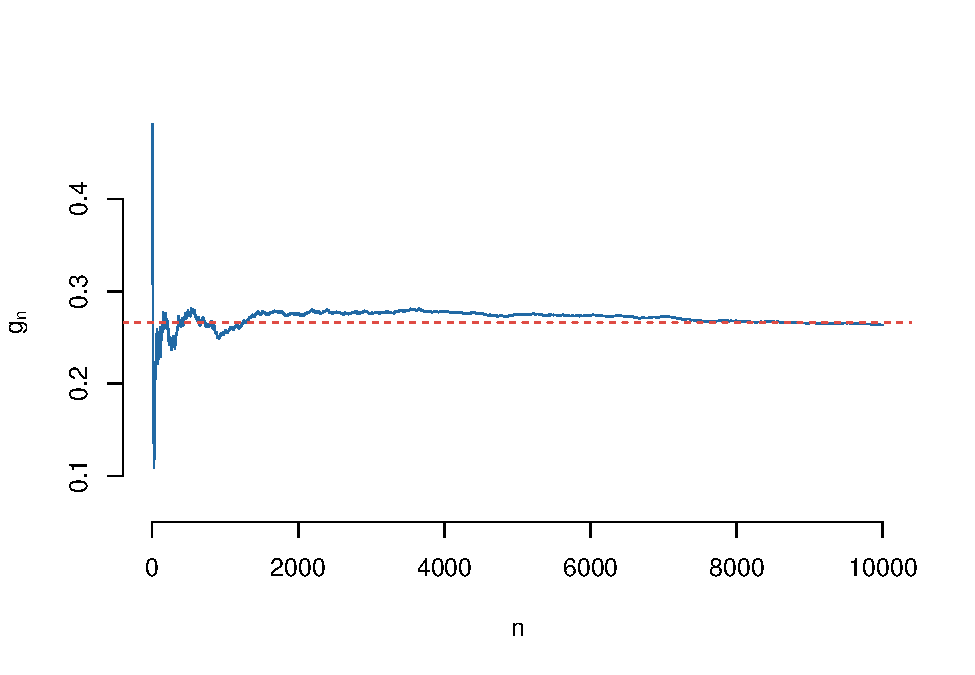
\includegraphics[width=0.8\linewidth]{Lab_2_files/figure-latex/unnamed-chunk-15-1} \end{center}

Observăm că probabilitatea de acoperire în acest caz este mai aproape de
ținta de \(1-\alpha = 0.95\) comparativ cu exemplul anterior.


\end{document}
